
% ----------------------------------------------------------------------
% Set the document class
% ----------------------------------------------------------------------
\documentclass[12pt]{article}
\usepackage{multirow}
% \usepackage{matlab-prettifier}
\usepackage[bordered]{uni-style}
\usepackage{uni-math}
\usepackage{pgfplots}
\usepackage{uni-code}

% ----------------------------------------------------------------------
% Define external packages, language, margins, fonts, new commands 
% and colors
% ----------------------------------------------------------------------
\usepackage[utf8]{inputenc} % Codification
\usepackage[english]{babel} % Writing idiom

\usepackage[export]{adjustbox} % Align images
\usepackage{amsmath} % Extra commands for math mode
\usepackage{amssymb} % Mathematical symbols
\usepackage{anysize} % Personalize margins
    \marginsize{2cm}{2cm}{2cm}{2cm} % {left}{right}{above}{below}
\usepackage{appendix} % Appendices
\usepackage{cancel} % Expression cancellation
\usepackage{caption} % Captions
    \DeclareCaptionFont{newfont}{\fontfamily{cmss}\selectfont}
    \captionsetup{labelfont={bf, newfont}}
\usepackage{cite} % Citations, like [1 - 3]
\usepackage{color} % Text coloring
\usepackage{fancyhdr} % Head note and footnote
    \pagestyle{fancy}
    \fancyhf{}
    \fancyhead[L]{\footnotesize \fontfamily{cmss}\selectfont Signals and Systems} % Left of Head note
    \fancyhead[R]{\footnotesize \fontfamily{cmss}\selectfont 25742} % Right of Head note
    \fancyfoot[L]{\footnotesize \fontfamily{cmss}\selectfont AIRLab} % Left of Footnote
    \fancyfoot[C]{\thepage} % Center of Footnote
    \fancyfoot[R]{\footnotesize \fontfamily{cmss}\selectfont Sharif University of Technology} % Right of Footnote
    \renewcommand{\footrulewidth}{0.4pt} % Footnote rule
\usepackage{float} % Utilization of [H] in figures
\usepackage{graphicx} % Figures in LaTeX
\usepackage[colorlinks = true, plainpages = true, linkcolor = istblue, urlcolor = istblue, citecolor = istblue, anchorcolor = istblue]{hyperref}
\usepackage{indentfirst} % First paragraph
\usepackage[super]{nth} % Superscripts
\usepackage{siunitx} % SI units
\usepackage{subcaption} % Subfigures
\usepackage{titlesec} % Font
    \titleformat{\section}{\fontfamily{cmss}\selectfont\Large\bfseries}{\thesection}{1em}{}
    \titleformat{\subsection}{\fontfamily{cmss}\selectfont\large\bfseries}{\thesubsection}{1em}{}
    \titleformat{\subsubsection}{\fontfamily{cmss}\selectfont\normalsize\bfseries}{\thesubsubsection}{1em}{}
    \fancyfoot[C]{\fontfamily{cmss}\selectfont\thepage}

% Random text (not needed)
\usepackage{lipsum}
\usepackage{duckuments}

% New and re-newcommands
\newcommand{\sen}{\operatorname{\sen}} % Sine function definition
\newcommand{\HRule}{\rule{\linewidth}{0.5mm}} % Specific rule definition
\renewcommand{\appendixpagename}{\LARGE \fontfamily{cmss}\selectfont Appendices}

% Colors
\definecolor{istblue}{RGB}{3, 171, 230}
\definecolor{dkgreen}{rgb}{0,0.6,0}
\definecolor{gray}{rgb}{0.5,0.5,0.5}

% Image path
\graphicspath{ {./Images/} }
%%%%%%%%%%%%%%%%%%%%%%%%%%%%%%%%%%%%%%%%%%%%%%%%%%%%%%%%%%%%%%%%%%%%%%%%
%                                 Document                             %
%%%%%%%%%%%%%%%%%%%%%%%%%%%%%%%%%%%%%%%%%%%%%%%%%%%%%%%%%%%%%%%%%%%%%%%%
\begin{document}

% ----------------------------------------------------------------------
% Cover
% ----------------------------------------------------------------------
\begin{center}
	\begin{figure}
		\vspace{-1.0cm}
		\centering
		
\includegraphics[scale = 0.15]{Images/Sharif_University_Logo.jpg} % IST logo
	\end{figure}
	\mbox{}\\[1.5cm]
	\textsc{\Huge \textbf{Signals and Systems Project}}\\[1.0cm]
	\textsc{\LARGE Instructor: Prof. Hamid Aghajan}\\[1.5cm]
	\textsc{\LARGE Sharif University of Technology}\\[1.0cm]
	\HRule\\[0.4cm]
	{\large \bf {\fontfamily{cmss}\selectfont Analysis of Phase Locking Value during Olfactory Stimulation \\ \medskip as a Biomarker for Alzheimer's Disease in EEG Signals} }\\[0.2cm]
	\HRule\\[1.5cm]
\end{center}

\begin{flushleft}
	\textbf{\fontfamily{cmss}\selectfont Authors:}
\end{flushleft}

\begin{center}
	\begin{minipage}{0.5\textwidth}
		\begin{flushleft}
			Alireza Gargoori Motlagh\\
			Mojtaba Lahijanian\\
			Amirali Loghmani\\
			S. Moienadin Makkiyan
		\end{flushleft}
	\end{minipage}%
	\begin{minipage}{0.5\textwidth}
		\begin{flushright}
			\href{mailto:alireza.gargoorimotlagh@ee.sharif.edu}{\texttt{alireza.gargoorimotlagh@ee.sharif.edu}}\\

			\href{mojtaba.lahijanian@ee.sharif.edu}{\texttt{mojtaba.lahijanian@ee.sharif.edu}}\\
			\href{mailto:amirali.loghmani@ee.sharif.edu}
			{\texttt{amirali.loghmani@ee.sharif.edu}}\\

			\href{mailto:moien.makkiyan@sharif.edu}{\texttt{moien.makkiyan@sharif.edu}}

		\end{flushright}
	\end{minipage}
\end{center}

\vspace*{0.5em}

\begin{flushleft}
	\textbf{\fontfamily{cmss}\selectfont Student, project by:}
\end{flushleft}

\begin{center}
	\begin{minipage}{0.5\textwidth}
		\begin{flushleft}
			Borna Khodabandeh
		\end{flushleft}
	\end{minipage}%
	\begin{minipage}{0.5\textwidth}
		\begin{flushright}
			\href{mailto:borna710kh@gmail.com}{\texttt{borna710kh@gmail.com}}\\
		\end{flushright}
	\end{minipage}
\end{center}

\begin{center}
	\bigskip \bigskip \bigskip \bigskip
	\large \bf \fontfamily{cmss}\selectfont Spring 2023
\end{center}

\thispagestyle{empty}

\setcounter{page}{0}

\newpage
\section*{Preface}
\textbf{\textsc{Notes} on the project:}
\begin{itemize}
	\item Due date: 1402/04/10 \medskip

	\item The project must be done individually. Each individual will present his results in an online session on 1402/04/11. \medskip

	\item Please submit your project report as a \texttt{.pdf} file. Include all outputs and final results in the report. Make sure to list the practice text questions and provide a concise explanation of your problem-solving approach in each section. \medskip

	\item Ensure that all codes are provided in a separate \texttt{.m/.py/.ipynb} file. If a code cannot be tested accurately upon submission, the reported results will be considered invalid, and no points will be awarded in such cases.\medskip

	\item You have the flexibility to utilize either \texttt{MATLAB} or \texttt{Python} for your project. However, please be aware that \texttt{MATLAB} is recommended since certain aspects of the project rely on \texttt{MATLAB} toolboxes.

	\item Ensure that you save all files, including your report, codes, helper functions, and any additional outputs, if required, in a compressed file format such as \texttt{.zip} or \texttt{.rar}. This compressed file should then be uploaded to the Coursework CW submission platform. \medskip

	\item Your file names must be in the following format: \begin{center}
		      \texttt{Project\_\#StudentID.zip/.rar/.pdf/.m/.py/.ipynb}
	      \end{center}
	      \medskip

	\item The details of the grading system of this project will be provided in the coming days. Generally, the project is worth a total of 1 point, with an additional 1 point allocated for the bonus section. Part 5.1 carries 0.5 points, and another 0.5 points are assigned to part 5.2. \medskip

	\item In this project, it is essential to uphold the principles of academic integrity and refrain from any form of cheating or copying. Cheating undermines the learning process, diminishes personal growth, and compromises the trust placed in us as students/researchers/professionals. It is crucial to recognize that engaging in dishonest practices not only tarnishes our own reputation but also has serious consequences, both ethically and academically. We want to emphasize that if anyone is found to have cheated, their results will not be accepted in this project, and they will receive a zero mark.

\end{itemize}
\newpage

% ----------------------------------------------------------------------
% Contents
% ----------------------------------------------------------------------
\tableofcontents

\newpage

% ----------------------------------------------------------------------
% Body
% ----------------------------------------------------------------------

% ------------------Section 1--------------------
\section{Introduction}
\subsection{Neurodegenerative Diseases} Neurodegenerative diseases, including Alzheimer's Disease (AD) and Mild Cognitive Impairment (MCI), pose significant challenges to individuals, families, and healthcare systems worldwide. These conditions are characterized by progressive deterioration of cognitive functions, leading to severe impairment and loss of independence. Understanding the importance of these diseases and the urgency to find reliable biomarkers for their early detection and accurate diagnosis is critical for effective intervention and disease management and has become a priority in the field of neurodegenerative research. \par
Alzheimer's disease, the most common form of dementia, affects millions of individuals globally, and its prevalence is expected to rise with the aging population. MCI, often considered a transitional stage between normal aging and AD, is characterized by subtle cognitive decline that does not severely impact daily functioning.
Scientists recognize that the combination of a person’s genes and environment contributes to their risk of developing a neurodegenerative disease. For example, someone might have a gene that makes them more susceptible to Parkinson’s disease, but their environmental exposures can affect whether, when, and how severely they are affected. \cite{ref-nih}

\subsection{Olfactory Dysfunction}
The sense of smell is today one of the focuses of interest in aging and neurodegenerative disease research. In several neurodegenerative diseases, such as Parkinson's disease and Alzheimer's disease, the olfactory dysfunction is one of the initial symptoms appearing years before motor symptoms and cognitive decline which manifests as a decreased ability to detect, identify, or differentiate odors and thus, being considered a clinical marker of these diseases' early stages and a marker of disease progression and cognitive decline. \cite{ref-olfactory} \par
One of the primary reasons olfactory dysfunction is prominent in neurodegenerative diseases is the presence of pathological changes in the olfactory system. In AD, for example, amyloid plaques and neurofibrillary tangles, the hallmark pathological features of the disease, are found not only in brain regions associated with memory and cognition but also in areas involved in olfaction, such as the olfactory bulb and olfactory cortex.

\subsection{Goal of the Project}
Understanding the significance of olfactory dysfunction in neurodegenerative diseases is important as it can serve as a potential biomarker for early detection and help unravel underlying disease mechanisms.
The study of olfactory dysfunction in neurodegenerative diseases is an active area of research. Researchers are investigating the potential of olfactory testing as a diagnostic tool and exploring the mechanisms underlying olfactory dysfunction. They are also examining the role of olfactory dysfunction in disease progression and exploring therapeutic interventions targeting the olfactory system. \par
In this project, we want to identify early biomarkers for related brain disorders through olfactory stimulus.
\newpage

% ------------------Section 2--------------------
\section{Electroencephalography (EEG)}
\subsection{What is EEG?}
There are different tools for collecting data from the brain. One of the methods of capturing brain signals is called Electroencephalography (EEG). These signals are changes in voltage level caused by changes in brain signals captured by some electrodes. These voltages are microVolt-level, so they can be sensitive to small noises. \par

One of the EEG advantages compared to other methods is its high temporal accuracy (i.e. high sampling frequency) while it suffers from low spatial accuracy. Another benefit of EEG devices is their smaller size compared to other devices like fMRI (functional Magnetic Resonance Imaging). While fMRI devices occupy the whole room, you can use EEG via portable devices.\par

EEG headsets are devices built to save EEG signals. These headsets could contain many electrodes. One internationally recognized electrode placement method is the \textbf{10-20 system}. This method was developed to maintain standardized testing methods ensuring that a subject's study outcomes (clinical or research) could be compiled, reproduced, and effectively analyzed and compared using scientific methods. It is called 10-20 because the distance between adjacent electrodes is 10\% or 20\%  of the skull's total front–back or right–left distance.

\begin{figure}[h]
	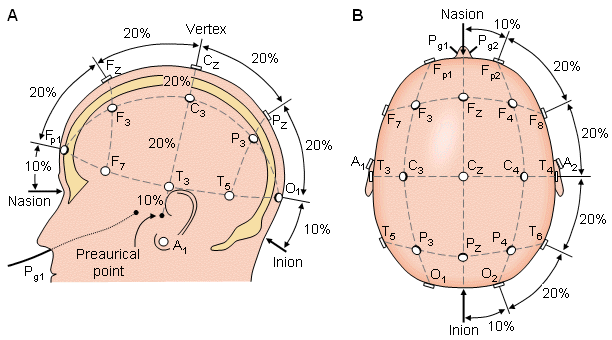
\includegraphics[scale=0.5,width=1\textwidth, inner]{EEG-10-20-Electrode-Placement}
	\caption{EEG 10-20 Electrode Placement System}
	\label{fig:figure1}
\end{figure}

Based on the picture above, What does each electrode's name stand for? Explain the naming method used in the 10-20 EEG system.

\begin{qsolve}[]
    The 10-20 EEG electrode placement system is a standardized method for positioning electrodes on the scalp for EEG recordings. Electrodes are named based on their anatomical locations using a combination of letters and numbers. The letters F, T, C, P, and O represent frontal, temporal, central, parietal, and occipital regions, respectively. The numbers indicate the distance between electrode placements and are based on percentages of specific measurements on the skull. For example, Fp1 and Fp2 electrodes are placed at 10\% and 20\% of the distance between specific landmarks on the skull. This naming method helps researchers and clinicians identify electrode locations and ensures consistent recording and comparison of EEG data across individuals and studies.
\end{qsolve}
% \newpage

\subsection{Alzheimer's Disease}
Alzheimer's Disease (AD) is a progressive and irreversible neurological disorder that affects the brain, primarily causing problems with memory, thinking, and behavior. It is the most common cause of dementia, a general term for a decline in cognitive ability severe enough to interfere with daily life. \par
The exact cause of Alzheimer's disease is not yet fully understood, but it is believed to involve a combination of genetic, lifestyle, and environmental factors. The staging of the AD is associated with the accumulation of Amyloid- beta ($A\beta$) proteins in the brain. These depositions cause synaptic and neuronal loss, which leads to major cognitive dysfunction in the advanced levels of the disease.\par

While EEG is not currently used as a primary treatment for Alzheimer's disease, it can be a valuable tool in the diagnosis and monitoring of the disease. EEG can help in the diagnosis of Alzheimer's by detecting abnormal patterns of brain activity that are characteristic of the disease. In individuals with AD, EEG often shows changes such as a reduction in certain brainwave frequencies and an increase in others. These patterns can aid in differentiating Alzheimer's from other types of dementia or cognitive disorders.

\subsection{Frequency Bands of EEG}
In the frequency domain, EEG signals are divided into 5 bands.\cite{freq-bands}

\begin{figure}[h]
	\centering
	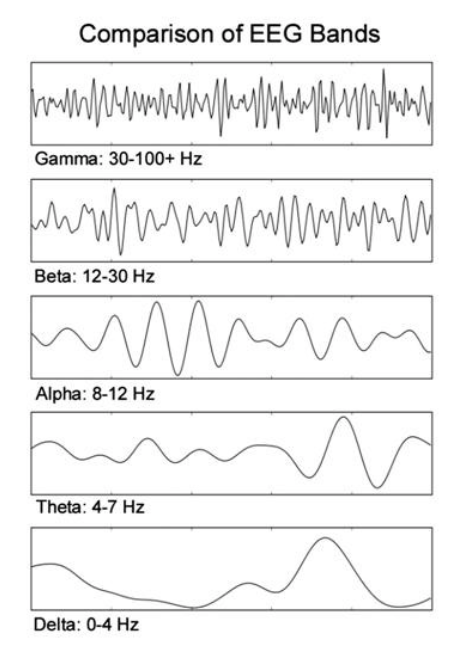
\includegraphics[scale=0.5]{freq-bands}
	\caption{EEG Frequency Bands}
	\label{ffig:figure2}
\end{figure}


\par
Determine the activities each frequency band is associated with.

\begin{qsolve}[]
	EG signals are divided into five frequency bands associated with specific activities:
	\begin{enumerate}
		\item Delta (0.5-4 Hz): Deep sleep, restorative processes, unconscious mind.
		\item  Theta (4-8 Hz): Light sleep, relaxation, meditation, memory formation, creativity.
		\item Alpha (8-12 Hz): Relaxation, closed eyes, wakeful relaxation, inhibition of distractions.
		\item Beta (12-30 Hz): Active mental states, alertness, problem-solving, decision-making.
		\item  Gamma (30-100 Hz): Cognitive processing, attention, memory retrieval, perception.
	\end{enumerate}
	These frequency bands represent different neural activities and cognitive processes observed in the brain. Understanding the associations between EEG frequency bands and specific activities provides insights into brain function and cognitive states.
\end{qsolve}

\newpage

\subsection{Sampling frequency}
Based on frequency bands and Nyquist criterion, which sampling frequencies are preferred for EEG signals?

\begin{qsolve}[]
	In order to accurately capture and analyze the intricate details of brain waves without introducing aliasing effects, it is essential to consider the maximum frequency of these waves.
	According to Figure \ref*{ffig:figure2}, the maximum frequency of brain waves is stated as 100Hz.
	To meet the requirements of the Nyquist rate, which states that the sampling frequency must be at least twice the maximum frequency of the signal, a minimum sampling frequency of 200Hz is necessary.
\end{qsolve}
\newpage

% ------------------Section 3--------------------
\section{EEG Signal Processing}
In this section, firstly you would get familiar with the task and the structure of the data.

\subsection{Task Definition}
\label{sec:sec3.1}
\cite{EEG-Dataset}
To identify the effect of olfactory dysfunction among different brain health states, the following task was performed to collect the data. The same sequence of stimuli was presented to all participants. The stimulation sequence was composed of two different odors, one occurring frequently (standard) with a probability of 0.75 and the other presented rarely (deviant) with a probability of 0.25. Each trial consisted of a 2s stimulus presentation followed by 8s of rest (pure water vapor). The odors were delivered to the participants using a laboratory olfactometer. The experiment involved 120 trials in which 90 frequent and 30 rare stimulation cycles were presented in a predetermined, randomized order. Lemon essence was used as the frequent odorant and rose essence was used as the rare odorant. These odors were selected to avoid trigeminal system activation as the olfactory and trigeminal systems are interconnected and may interact with each other during exposure to certain stimuli \cite{olfactory-trigeminal}. The duration of odor presentation was set at 2s to enable regular breathing cycles for the participants.

\subsection{Data Description}
\label{sec:sec3.2}
\cite{EEG-Dataset}
The dataset consists of three files as follows:

\begin{itemize}
	\item \texttt{AD.mat}: Contains data for Alzheimer’s disease patients.
	\item \texttt{Normal.mat}: Contains data for healthy elderly participants.
	\item \texttt{MCI.mat}: Contains data for mild cognitive impairment patients. (Described in part \hyperref[sec:5.1]{5.1})
\end{itemize}

The structure of the files is the same. Each file is organized as a structure array, in which each row contains information of one participant and the three columns correspond to the “epoch”, “odor” and “noisy” fields as described in Table 1.


\begin{table}[]
	\begin{center}
		\begin{tabular}{  | l | p{13cm} |}
			\hline
			Field & Description                                                                                                                                                                                                                                                                                                                                                                                                                                               \\
			\hline
			epoch & This is a 3D array structured as 4 × 600 × Num\_trials. The first dimension indicates EEG channels respectively from the first column as Fp1, Fz, Cz, and Pz. The second dimension contains EEG samples from 1 s pre stimulus to 2 s post stimulus, which at a 200 Hz sampling rate amounts to 600 samples. The last dimension shows the number of trials. This could be different for each participant as some trials were deleted during preprocessing. \\
			\hline
			odor  & This is a 2D binary array shaped as Num\_trial × 1. This array shows the odorant type (lemon/rose) the participant was exposed to in each trial. The value = 1 indicates the rose odor and the value = 0 indicates the lemon odor.                                                                                                                                                                                                                        \\
			\hline
			noisy & This is a 2D array with the size 1 × Num\_noisy. This array indicates noisy trials identified based on comparing the instantaneous and average trial amplitudes. These noisy trails can be ignored in processing and were included for the dataset completeness.                                                                                                                                                                                          \\
			\hline
		\end{tabular}
		\label{tab:table1}
	\end{center}
	\caption{Description of each structure array (.mat file) in the dataset.}
	\label{table:Data-Structure}


\end{table}
\newpage


\subsection{Pre-Processing}
Using a standard pipeline in EEG signal preprocessing is crucial for ensuring consistency, reproducibility, and objectivity in research. It reduces bias, enhances the reliability of results, and provides established best practices for addressing common challenges. A popular and widely used pipeline for EEG signal preprocessing is Makoto's pipeline (\href{https://sccn.ucsd.edu/wiki/Makoto's_preprocessing_pipeline}{\texttt{Makoto’s preprocessing pipeline - SCCN}}).\\

The collected raw data from all participants were preprocessed following the full pipeline of Makoto with the use of EEGLAB and posted as a dataset, as described in the following steps:

\begin{enumerate}
	\item  Apply 1 Hz high pass filter to remove baseline drifts.
	\item  Apply relevant notch filter to remove the 50 Hz line noise.
	\item  Reject bad channels as a critical step before average referencing with the use of \texttt{clean\_rawdata()} EEGLAB plugin.
	\item  Interpolate the removed channels.
	\item  Re-reference the data to the average of all channels to obtain a good estimate of referenceindependent potentials.
	\item  Apply \texttt{clean\_rawdata()} for cleaning the data by running artifact subspace reconstruction(ASR).
	\item  Re-reference the data to the average again to compensate for any potential changes in the data caused by the previous step.
	\item  Run independent component analysis (ICA) to identify EEG sources as well as the sources associated with noise and artifacts.
	\item  Fit single and bilateral (if available) current dipoles.
	\item  Further clean the data by source (dipole) selection using \texttt {IClabel()} plugin in EEGLAB.
\end{enumerate}

In the \texttt{Dataset/Preprocess} folder you can find the raw data for 2 subjects with the corresponding additional information provided. In this section you are required to preprocess these data and save your final preprocessed cleaned data.\\
However, there is no need to fully implement the Makoto's pipeline and a simplified version of this is as follows; follow the instructions below and provide the required results in each step:\\
\begin{figure}[h]
	\center 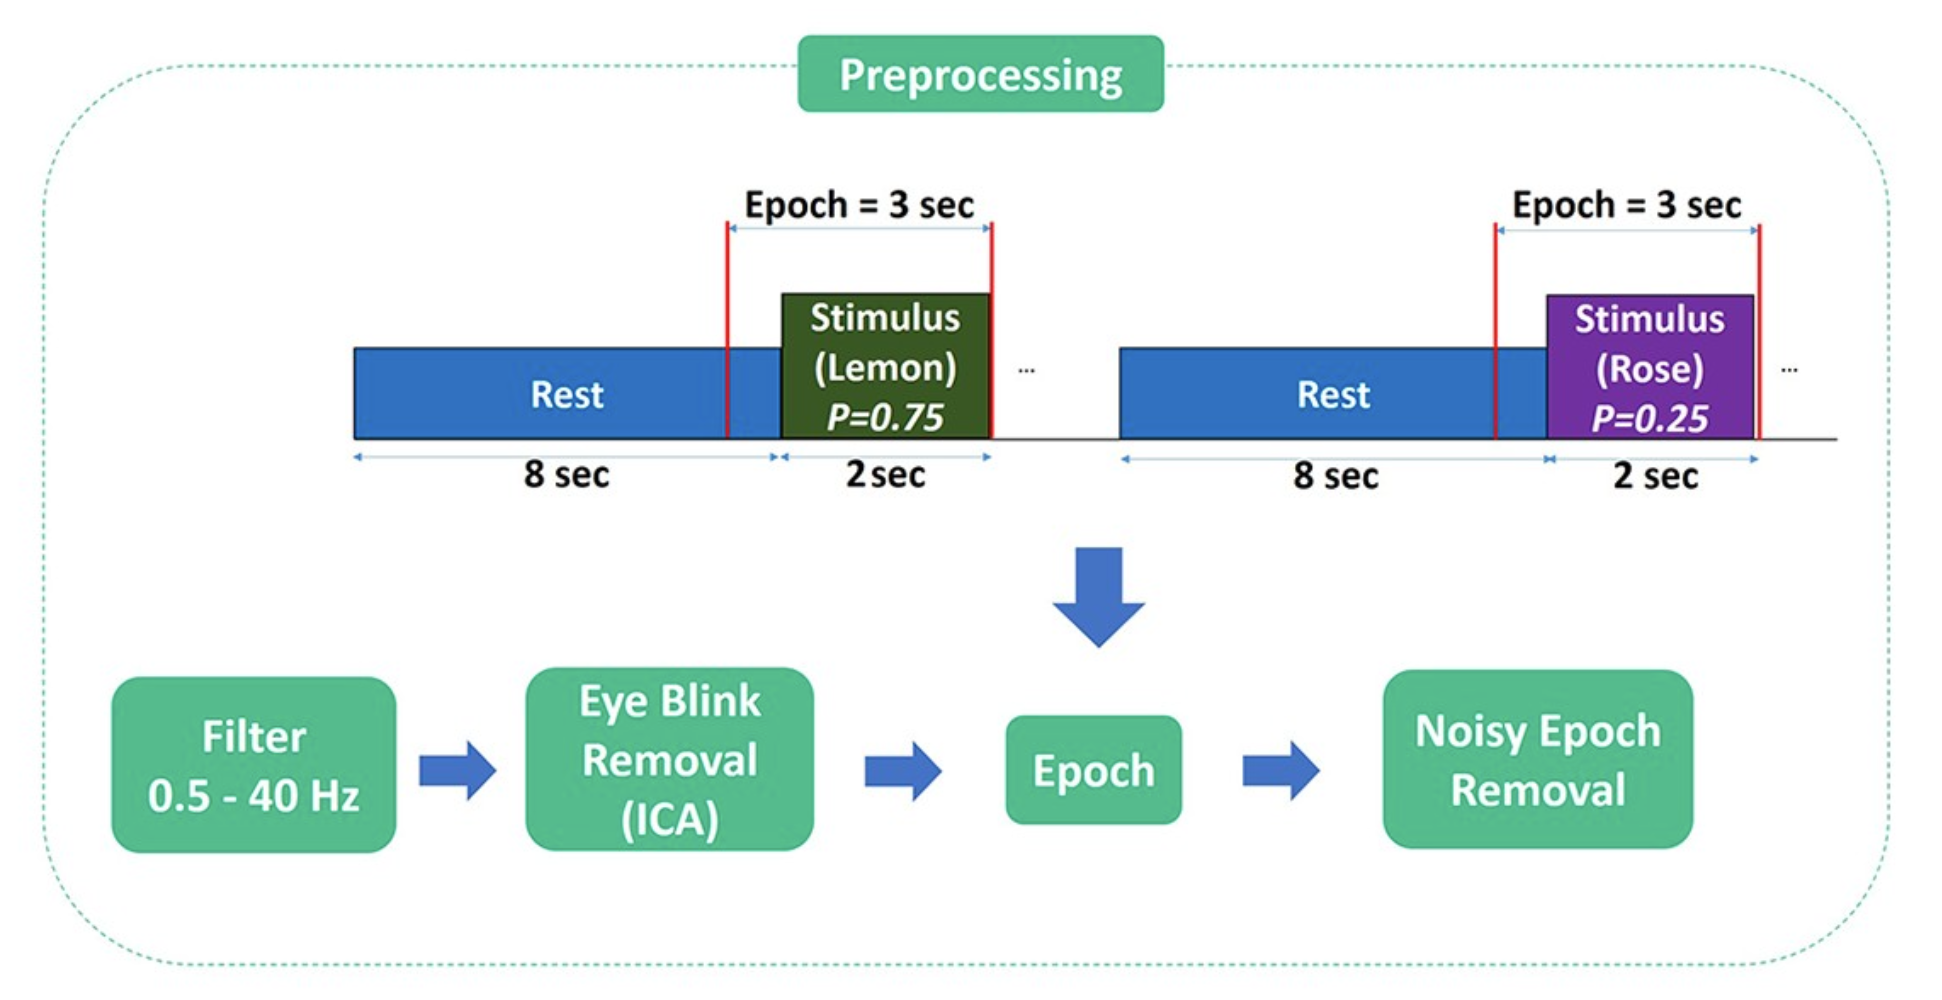
\includegraphics[scale=1,width=0.8\textwidth]{Images/Preprocess.png}
	\caption{Task and Preprocessing Steps \cite{olfactory-deficit-AD}}
	\label{fig:fig3}
\end{figure}
\begin{itemize}
	\item \textbf{Step 1}: To preproccess using EEGLAB, first re-reference data to the mean of the channels. Then use a bandpass filter to filter 0.5 - 40.5 Hz frequencies. As we have filtered to 40.5 Hz, there is no need to apply a 49.9 - 50.1 Hz notch filter to remove the line noise (However, keep this step in mind as this is a crucial step in EEG signal preprocessing!). Using FFT function or EEGLAB, plot the frequency spectrum of \texttt{Fz} channel data. (Just to note, your data will be saved at EEG struct in MATLAB workspace.)\\

	\item \textbf{Step 2}: In this part you would remove the artifacts of the signal. Artifacts include blinking, eye movement, muscle movement, heart rate and etc. For this, load your data at EEGLAB. Now load \texttt{Standard-10-20-Cap19.loc} file from \texttt{edit-channel loacations} menu that contains locations of channels. Then run ICA (Independent Component Analysis) algorithm from \texttt{tools-decompose data} by ICA menu. Please note that this part would probably takes more time. Then you will have the a figure like \hyperref[fig:fig4]{Figure 4} by running \texttt{tools $\rightarrow$ classify components using ICLabel-label components.}
	      \begin{figure}[h]
		      \center 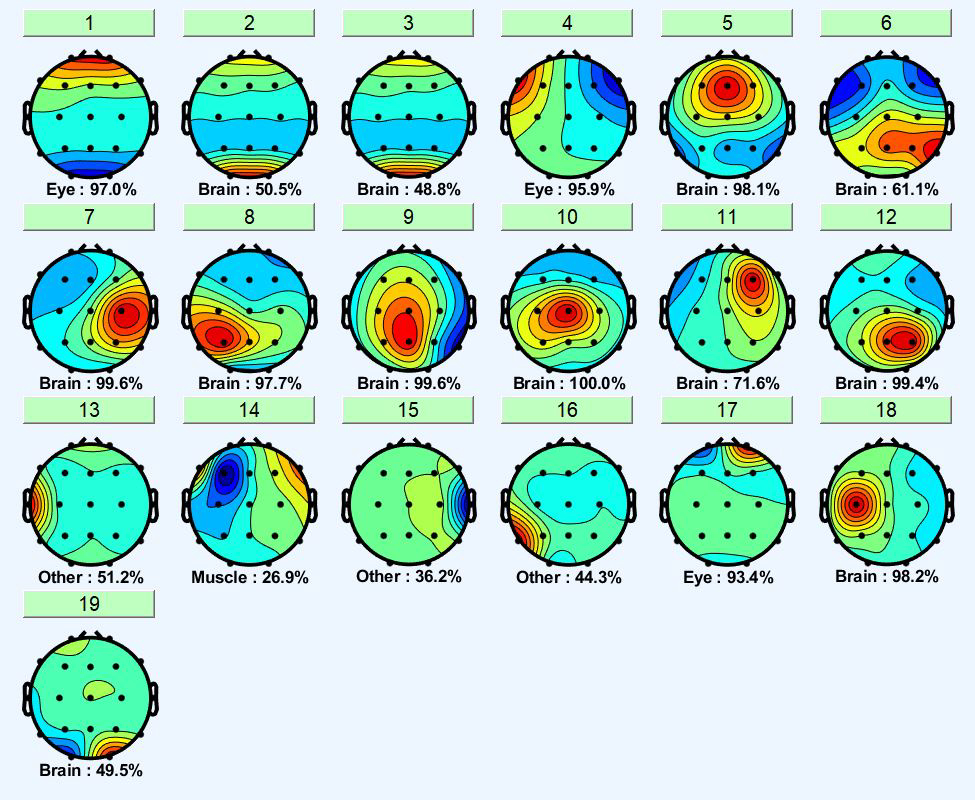
\includegraphics[scale=1,width=0.6\textwidth]{Images/brain_map.jpg}
		      \caption{An example of ICA components}
		      \label{fig:fig4}
	      \end{figure}
	      By clicking on each component, you can some details about it as well. Present a figure from one of the brain components with its details. \par
	      Now remove all non-brain components. For this purpose, from \texttt{Tools-remove components from data} enter the number of components that must be removed. \\

	\item \textbf{Step 3}:  Epoch the data of each subject. Epoch is a 3D matrix of the shape \{\texttt{Num\_Channels $\times$ Samples $\times$ Num\_Trials}\}. In fact, all data must be reshaped as the following figure suggests:
	      \begin{figure}[h]
		      \center 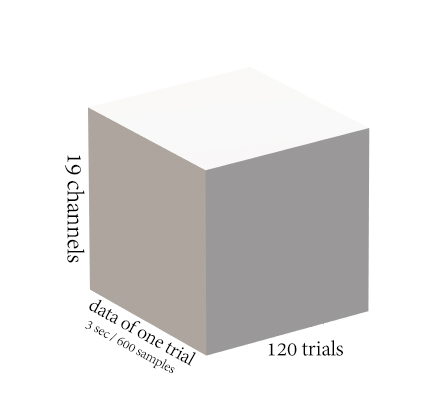
\includegraphics[scale=1,width=0.4\textwidth]{Images/epoch.jpg}
		      \caption{Epoch}
		      \label{fig:fig5}
	      \end{figure}\\
	      For epoching the data, starting point of the experiment is required. This is provided in the \texttt{help} file for each subject. Please note that you must epoch the data by considering this time as the start. Also, the data after 120 trials should be neglected as well.

	\item \textbf{Step 4}: In this step, you need to remove noisy trials. There are two ways to achieve this:
	      \begin{enumerate}
		      \item Observe data at EEGLAB and remove any trial that seems noisy. (\textsc{Preferred!})
		      \item Using power spectrum of each trial, remove trials that their standard deviation of their power spectrum is bigger than 3.5 .Create a 3D matrix by each trial's power spectrum for each channel using \texttt{pspectrum} in MATLAB. You can use the following commands to find noisy trials:
		            \begin{lstlisting}[style=Matlab-editor]
vr = sum(nanstd(p,[],2).^2,2);
noisy_trials = find(abs(zscore(vr))>3.5);
        \end{lstlisting}

		            In these commands, \texttt{p} is a matrix of frequency spectrums of all trials of a channel. \texttt{noisy\_trials} contains the number of noisy trials of that channel. These commands must run for each channel individually and the resultant noisy trials must be accumulated over all channel. Then remove all \texttt{noisy\_trials} from your epoch.
	      \end{enumerate}

	\item \textbf{Step 5}: In the final step, only subsample the data corresponding to the \texttt{Fp1, Fz, Cz \& Pz} channels. You can find the channels' orders in the \texttt{Channels.jpg}.
\end{itemize}

Do these 5 steps for each subject and save the final data through an \texttt{struct} with the same format as described in \hyperref[tab:table1]{Table 1}. Also, consider the order of \texttt{odor} being the same as the ones used for normal participants.

\begin{qsolve}[]
	the process is followed and the final data is stored in the project \texttt{preprocessing} directory.

	snapshots of the process for subject 1 follow:
\end{qsolve}

\vfil
\begin{figure}[h!]
	\centering
	\includegraphics*[width=\linewidth]{../computation/preprocessing/snapshots/subject1.png}
	\caption{starting point}
\end{figure}

\newpage

\begin{figure}[h]
	\centering
	\includegraphics*[width=\linewidth]{../computation/preprocessing/snapshots/power_spectrum_Fz.png}
	\caption{Frequency spectrum for the Fz channel}
	\includegraphics*[width=0.49\linewidth]{../computation/preprocessing/snapshots/ICA_Labels.png}
	\includegraphics*[width=0.49\linewidth]{../computation/preprocessing/snapshots/ICA_brain_only.png}
	\caption{ICA labeling}
\end{figure}

\vfil
\begin{qsolve}[]
	we remove noisy epochs using the given toolboxes in EEGLAB
\end{qsolve}
% \newpage

\begin{figure}[h]
	\includegraphics*[width=\linewidth]{../computation/preprocessing/snapshots/noisy_epoch.png}
	\caption{noisy epoch removal}
\end{figure}


\clearpage
\newpage

\subsection{Phase Locking Value (PLV)}
\label{sec:3.4}
Phase Locking Value (PLV) is a metric used to quantify the degree of phase synchronization or phase consistency between two oscillatory signals. It assesses the relationship between the phases of two signals at a specific frequency range. PLV is commonly used in the analysis of neural signals, including electroencephalography (EEG) and magnetoencephalography (MEG), to investigate the synchronization of oscillatory activity between different brain regions or across different frequency bands within a single region.. It provides insights into the functional connectivity and coordination of neural activity. \par

\medskip
PLV ranges from 0 to 1, where a value of 1 indicates perfect phase synchronization, while a value close to 0 represents a lack of synchronization. High PLV values suggest that the phases of the two signals are consistently aligned or coupled, indicating strong synchronization. This synchronization can reflect functional interactions between brain regions or coordinated activity within a network. In contrast, low PLV values indicate weaker or desynchronized activity, suggesting less functional coupling between the signals.\par

\begin{itemize}
	\item What does phase synchronization indicate from a functional point of view? Discuss its importance with valid references. \begin{qsolve}[]
		      Phase synchronization, as indicated by the Phase Locking Value (PLV), carries important functional implications in the study of neural activity and brain function. It provides insights into the coordination and communication between different brain regions or within a single region. By analyzing the phase synchronization between oscillatory signals, researchers can uncover the functional connectivity and interactions that underlie various cognitive processes.

		      \vspace*{1em}
		      The functional significance of phase synchronization lies in its association with information transfer and integration across brain regions. Synchronized oscillatory activity enables the coordination of neural firing and facilitates the communication and integration of information between different regions.
	      \end{qsolve}\medskip

	\item Formulate the definition of PLV and briefly discuss the mathematical tools needed to calculate it. \begin{qsolve}[]
		      The PLV is typically calculated using the following formula:
		      \[
			      PLV = |E(e^{i\Delta{\Phi(t)}})| ,\quad \Delta{\Phi(t)}=\Phi_1(t) - \Phi_2(t)
		      \]
		      where $\Phi$ is the phase of the signal, more percsisely the phase of the analytical signal, where
		      the analytical signal is defined by the following formula:

		      \[
			      z(t) = s(t) + ih(t),\quad h(t)=\mathbb{H}(s(t))=\frac{1}{\pi}\intinf \frac{s(\tau)}{t-\tau}d\tau
		      \]

		      \cite[reference]{Phase-locking-value}
	      \end{qsolve}
	      \medskip

	\item Implement a function which finds the PLV between two channels in a specific frequency range. This function is going to be needed in the \hyperref[sec:sec4]{section 4}. (\textsc{Note}: You are allowed to define this function with any required input arguments.)   \begin{qsolve}[]
		      here is the implementation of this function in matlab.

	      \end{qsolve}
\end{itemize}


\begin{lstlisting}[style=matlab-editor]
function plv = PLV(signals1, signals2, fs, bandwidth)
    if nargin < 4
        bandwidth = [0.001 fs/2-0.001]; % Default to all-pass filtering
    end
    
    numSignals = size(signals1, 3);
    plv = zeros(1, numSignals);
    
    for i = 1:numSignals
        signal1 = signals1(:,:,i);
        signal2 = signals2(:,:,i);

        % filtering the signal to the desired bandwidth
        filteredSignal1 = bandpass(signal1, bandwidth, fs);
        filteredSignal2 = bandpass(signal2, bandwidth, fs);
        
        % calculating phase difference
        phaseDiff = phase_diff(filteredSignal1, filteredSignal2);

        % Calculate the PLV
        plv(i) = abs(mean(exp(1j * phaseDiff)));
    end
end

function phaseDiff = phase_diff(signal1, signal2)
    analytic1 = hilbert(signal1);
    analytic2 = hilbert(signal2);
    phase1 = angle(analytic1);
    phase2 = angle(analytic2);
    phaseDiff = phase1 - phase2;
end\end{lstlisting}
\newpage



% ------------------Section 4--------------------
\section{Results}
\label{sec:sec4}
In this section, you need to present the required results to assess the difference of Phase Locking Values (PLV) among two groups, namely AD and Normal in the slow gamma frequency range, which is 35 to 40 Hz.\par \medskip
To fairly compare your results in this part, you do not need to use your preprocessing data from section \hyperref[sec:sec3.3]{3.3} and the preprocessed data of 15 healthy (normal) (age = 69.27±6.65, female = 53.33\%) individuals and 13 AD patients (age = 75.31±9.90, female = 61.54\%) are availabe through \texttt{Dataset/Normal.mat} and \texttt{Dataset/AD.mat}.\\


\subsection{Values} Find the PLV for all participants of both groups on both frequent and rare odors between the \texttt{Fz} and \texttt{Cz} channels using the function you implemented in section \hyperref[sec:3.4]{3.4} . \begin{qsolve}[]
	To calculate the Phase Locking Value (PLV) between the specified channels for each participant, we employ the following procedure:

	Firstly, we utilize different epochs and determine the average signal for Fz and Cz in each trial. This step helps in mitigating any temporal effects by averaging out activities other than the stimulus. By computing the mean of the signal, we obtain a signal that solely represents the impact of the stimulus, effectively removing extraneous variations.

	Subsequently, we proceed to calculate the PLV between the Fz and Cz channels for each participant, distinguishing between rare and frequent stimuli. The resulting PLV values are then stored in an array, enabling further analysis and interpretation.

	For instance, when considering normal patients, the code implementation follows as follows:
\end{qsolve}
\begin{lstlisting}[style=matlab-editor,basicstyle=\small]
for p = 1:numNormalPatients
    % Extract relevant data for the current Normal patient
    person = normal(p);
    rare = person.epoch(:,:,logical(person.odor));
    frequent = person.epoch(:,:,~logical(person.odor));
    Fz_Cz_rare = squeeze(rare(2:3,:,:));
    Fz_Cz_frequent = squeeze(frequent(2:3,:,:));
    % Calculate PLV for rare trials
    Fz_mean = mean(Fz_Cz_rare(1,:,:),3);
    Cz_mean = mean(Fz_Cz_rare(2,:,:),3);
    mean_plv_rare_Normal(p) = PLV(Fz_mean,Cz_mean,sampling_rate,bandwidth);
    % Calculate PLV for frequent trials
    Fz_mean = mean(Fz_Cz_frequent(1,:,:),3);
    Cz_mean = mean(Fz_Cz_frequent(2,:,:),3);
    mean_plv_frequent_Normal(p) = PLV(Fz_mean,Cz_mean,sampling_rate,bandwidth);
end\end{lstlisting}
\medskip

\subsection{Distributions} Draw the box plots of PLVs you found in the previous part among two groups and two odors. Also, fit a gaussian distribution on these PLVs and present you results. You need to specify the corresponding \texttt{p-values} to evaluate the statistical significance of your findings.
\begin{qsolve}[]
	after finding the plv for each event, we simply draw a box plot of the plv values to see if the values are different.

	after that, we just use the matlab \texttt{fitdist} and then \texttt{ttest2} functions in \textsc{matlab} to test significance and to fit a gaussian distribution to our findings.
\end{qsolve}
\begin{figure}[h]
	\centering
	\includegraphics*[width=\linewidth]{../computation/PLV/result/boxplot.png}
\end{figure}
\begin{figure}[h]
	\centering
	\includegraphics*[width=\linewidth]{../computation/PLV/result/gaussian_fit.png}
	\caption{fitting gaussian distributions}
\end{figure}
\medskip

\subsection{Statistical Significance} Based on the \texttt{p-values} you founded in the previous part, discuss whether we could state that the "PLV is significantly different among AD and Normal subjects in the slow gamma frequency range".
\begin{qsolve}[]
	by the results of the \texttt{ttest2}, we could say that:
	\begin{center}
		``\textbf{
			for rare trials, PLV is significantly different among AD and Normal subjects in the slow gamma frequency range ( p = 0.037 )
		}"

		``\textbf{
			for frequent trials, PLV is most likely different among AD and Normal subjects in the slow gamma frequency range ( p = 0.156 )
		}"
	\end{center}
\end{qsolve}\medskip

\subsection{Phase Difference} Draw a polar histogram of the phase difference between \texttt{Fz} and \texttt{Cz} channels during frequent odor trials for a random subject in each group and compare the results. Also, plot the mean value of this quantity among all the subjects of each group and discuss the results.
\begin{qsolve}[]
	Using the previously defined phase difference for calculating the PLV between the two signals, we construct a histogram that represents the distribution of this phase difference. This histogram captures the accumulated phase data for all participants within each group, pertaining to each odor condition.

	Essentially, this histogram provides a visual representation of the collective phase information for all participants in a given group, highlighting the variations and patterns in the phase differences between the signals. By examining the histogram, we can gain insights into the synchronization or desynchronization of the signals, allowing for a deeper understanding of the neural responses to different odors within each group.

	as seen from the data, the AD patients have more sparse phase patterns.
\end{qsolve}

\begin{figure}[h]
	\centering
	\includegraphics*[width=\linewidth]{../computation/PLV/result/phase_diff.png}
\end{figure}

\subsection{Heatmaps} Now you need to plot a heatmap which has the PLVs between each pair of the channels. Find whether PLV between other channel pairs are significantly different among two groups in the slow gamma frequency range and test your results. (\textsc{Note:} You need to provide \texttt{p-values} for your hypothesis if you found any significantly different channel pairs apart from (\texttt{Fz},\texttt{Cz}).)

\begin{qsolve}[]
	here, we do the same kind of analysis we did before for calculating the plv between Fz, Cz channels.
	here we take the mean of the PLV between all participants.

	The PLV matrix represents the average Phase Locking Value (PLV) between each pair of channels for a group of normal patients. Mathematically, the PLV between two channels, denoted as channels $i$ and $j$, is calculated as follows:

	\[
		PLV_{ij} = \frac{1}{M} \sum_{m=1}^{M} \Big|\frac{1}{N} \sum_{n=1}^{N} e^{i(\phi_i^{m,n} - \phi_j^{m,n})}\Big|
	\]

	where:
	\begin{itemize}
		\item $PLV_{ij}$ represents the PLV value between channels $i$ and $j$.
		\item $M$ is the total number of normal patients.
		\item $N$ is the number of trials per patient.
		\item $\phi_i^{m,n}$ and $\phi_j^{m,n}$ are the instantaneous phase values of channels $i$ and $j$ in the $n$th trial of the $m$th patient, respectively.
	\end{itemize}

	as seen from the results, the Fz, Cz channels indeed show the most significant difference in the PLV, so we conclude that Fz, Cz are the most different channels.
	the results follow:
\end{qsolve}

\begin{figure}[h]
	\centering
	\includegraphics*[width=\linewidth]{../computation/PLV/result/heatmap.png}
\end{figure}
\newpage

% ------------------Section 5--------------------
\section{$^*$Bonus}
\subsection{Mild Cognitive Impairment (MCI)}
\label{sec:5.1}
Mild Cognitive Impairment (MCI) is the stage between the expected decline in memory and thinking that happens with age and the more serious decline of dementia. MCI may include problems with memory, language or judgment. People with MCI may be aware that their memory or mental function has slipped. \cite{mayo-MCI}
\begin{figure}[h]
	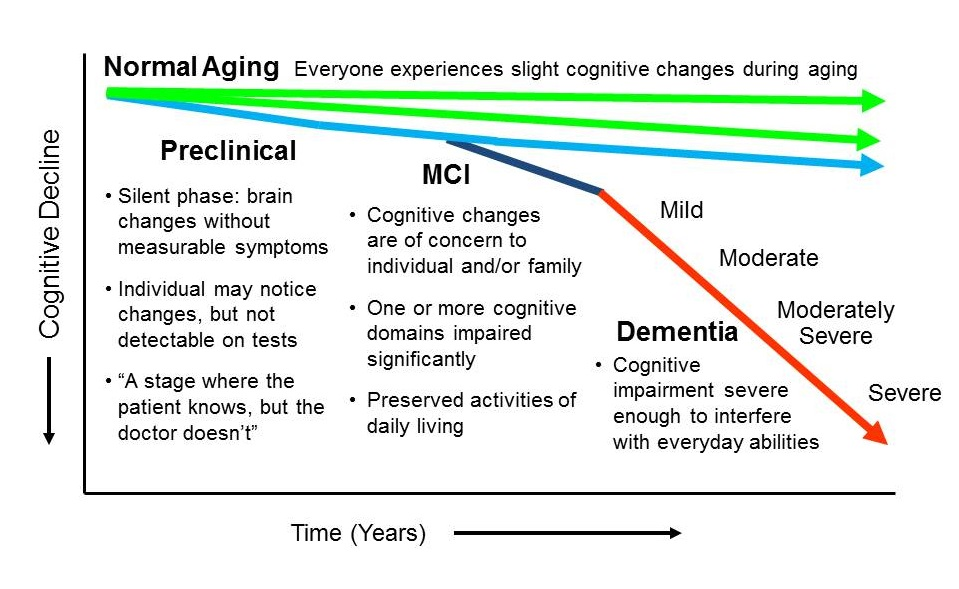
\includegraphics[scale=0.5,width=1\textwidth, inner]{Normal-aging-to-dementia.jpg}
	\caption{Normal Aging to Demantia Process}
	\label{fig:figure2}
\end{figure}

\subsubsection{Additional Information}
Describe the relationship between MCI and AD. Explain whether MCI would always result in AD and briefly investigate the causes of MCI.

\begin{qsolve}[]
	MCI is a stage characterized by mild cognitive decline that is greater than expected for age but does not meet the criteria for dementia. While MCI increases the risk of developing AD, it does not always lead to AD, and some individuals with MCI may remain stable or even improve over time. The causes of MCI are diverse and can include age-related changes, vascular issues, neurodegenerative diseases, genetic factors, and lifestyle/environmental factors.
\end{qsolve}

\subsubsection{MCI Data Processing}
In the provided dataset, you can find \texttt{MCI.mat} file. This dataset contains preprocessed cleaned EEG recording of the same task described in sections \hyperref[sec:sec3.1]{3.1} and \hyperref[sec:sec3.2]{3.2} for 7 MCI patients. \par
Based on the significantly different coupled channels you found for differentiation between AD and Normal groups, find the Phase-Locking-Value (PLV) for the MCI subjects and provide the required results by comparing all the the 3 states (Normal, MCI, AD). Your findings must include the significance testing by providing the corresponding \texttt{p-values}.

\begin{qsolve}[]
	here we apply the same methods we used in the previous section, the results follow:
	due to limited number of MCI subjects, the p-values don't show much significance.

	\begin{center}
		``\textbf{
			for rare trials, PLV is most likely different among AD and MCI subjects in the slow gamma frequency range ( p = 0.17 )
		}"

		``\textbf{
			for frequent trials, PLV is significantly different among AD and MCI subjects in the slow gamma frequency range ( p = 0.045 )
		}"

		``\textbf{
			for rare trials, PLV might be different among Normal and MCI subjects in the slow gamma frequency range ( p = 0.74 )
		}"

		``\textbf{
			for frequent trials, PLV might be    different among Normal and MCI subjects in the slow gamma frequency range ( p = 0.69 )
		}"
	\end{center}
\end{qsolve}

\begin{figure}[h]
	\centering
	\includegraphics*[width=\linewidth]{../computation/MCI/results/boxplot_MCI.png}
\end{figure}

\subsection{Phase-Amplitude Coupling (PAC)}
PLV was just one instance of the Phase-Amplitude Coupling (PAC) metrics. PAC is a form of cross-frequency coupling where the amplitude of a high frequency signal is modulated by the phase of low frequency oscillations. PAC is the most-studied type of cross-frequency coupling and is thought to be responsible for integration across populations of neurons. Low frequency brain activity controls the information exchange between brain regions by modulating the amplitude of the high frequency oscillations.\cite{PAC-nature}



\subsubsection{Metrics}
Conduct a search about other PAC measures and briefly provide an explanation about two of them.

\begin{qsolve}[]
	\begin{itemize}
		\item Phase-locking value (PLV): This is a measure of the consistency of the phase difference between two signals at a given frequency. It ranges from 0 to 1, with 1 indicating perfect phase locking.
		\item Mean vector length (MVL): This is a measure of the strength and direction of the coupling between two signals. It ranges from 0 to 1, with 1 indicating perfect coupling.
		\item Modulation index (MI): This is a measure of the degree to which the amplitude of one signal is modulated by the phase of another signal. It ranges from -1 to 1, with 0 indicating no modulation.
		\item Generalized linear modeling cross-frequency coupling (GLM-CFC): This is a method that uses a generalized linear model to estimate the strength and direction of coupling between two signals at different frequencies.
	\end{itemize}\cite{10.3389/fnins.2019.00573}
	here we arbitrary chose to implement the modulation index.
\end{qsolve}
\subsubsection{Implementation}
Implement one of the metrics mentioned earlier as a biomarker for distinguishing between AD and Normal groups. Present the relevant results through plots and provide a discussion regarding the efficacy of the selected metric.
\\

\begin{qsolve}[]
	here we arbitrary chose to implement the modulation index, sadly the results were not very significant for
	any of the channels.
\end{qsolve}

\begin{lstlisting}[style=matlab-editor, basicstyle=\small]
function MI = modulation_index(x, fs, bandwidth, num_bins)
    if nargin < 3
        bandwidth = [0.001 fs/2-0.001]; % Default to all-pass filtering
    end if nargin < 4
        num_bins = 18; % Default to 18 bins
    end
    numSignals = size(x, 1);
    MI = zeros(1, numSignals);
    for i = 1:numSignals
        signal = x(i,:,:);
        % Filtering the signal to the desired bandwidth
        filteredSignal = bandpass(signal, bandwidth, fs);
        analyticSignal = hilbert(filteredSignal);
        % Calculate the phase and amplitude of the analytic signal
        phase = angle(analyticSignal);
        amplitude = abs(analyticSignal);
        % Bin the phase values into the specified number of bins
        bins = linspace(-pi, pi, num_bins+1);
        phase_bins = discretize(phase, bins);
        % Convert phase_bins to numeric array
        phase_bins = double(phase_bins);
        % Calculate the average amplitude in each phase bin
        avg_amplitude = zeros(num_bins, 1);
        for j = 1:num_bins
            values = amplitude(phase_bins == j);
            if ~isempty(values)
                avg_amplitude(j) = mean(values);
        end end
        % Normalize the average amplitudes
        normalized_amplitude = avg_amplitude / sum(avg_amplitude);
        % Calculate the Shannon entropy
        entropy=-sum(normalized_amplitude.*log2(normalized_amplitude));
        % Calculate the Kullback-Leibler distance
        KL_distance = log2(num_bins) - entropy;
        MI(i) = KL_distance / log2(num_bins);
    end
end\end{lstlisting}

\begin{figure}[h!]
	\centering
	\includegraphics*[width=\linewidth]{../computation/MCI/results/boxplot_MI.png}
	\caption{findings for the MI index of each channel}
\end{figure}

% ------------------Section 6--------------------
\section{Conclusion}
In this section, you are required to thoroughly examine and analyze the results you have obtained throughout this project. You must provide a comprehensive discussion of your findings, highlighting their significance and relevance to the research question. You should also present any limitations or weaknesses in your study and suggest possible areas for future research. Overall, this section is critical to demonstrating the quality and validity of your research and should be approached with careful attention to detail and clarity of expression.

% \begin{qsolve}[]
    \vfil
	\begin{conclusion}

		In summary, our study aimed to investigate phase-amplitude coupling using different metrics, including the Phase Locking Value (PLV), Modulation Index (MI), and Generalized Linear Model-Phase Coupling Factorization (GLM-CFC).

		When analyzing the PLV, we observed significant differences between groups in the slow gamma frequency range. Specifically, for rare trials, the PLV was significantly different between AD and Normal subjects (p = 0.037), while for frequent trials, the PLV showed significant differences between AD and MCI subjects (p = 0.045). However, the significance of the findings was limited due to the small number of MCI subjects.

		Although we implemented the modulation index, the results did not yield significant findings for any of the channels studied. This suggests that phase-amplitude coupling, as measured by the modulation index, may not play a prominent role in the observed differences between groups.

		Furthermore, we analyzed the PLV matrix to examine the average PLV between channels for a group of normal patients. The Fz and Cz channels exhibited the most significant differences in PLV, indicating that these channels are the most distinct among the measured pairs.

		Due to the limited number of MCI subjects in our study, the p-values obtained did not show significant differences. However, the results suggest potential differences in PLV between AD and MCI subjects in the slow gamma frequency range. Specifically, for rare trials, the PLV is most likely different between AD and MCI subjects (p = 0.17), while for frequent trials, the PLV is significantly different between AD and MCI subjects (p = 0.045).

		It is important to acknowledge the limitations of our study, including the small number of MCI subjects and the arbitrary choice of the modulation index. Future research should explore alternative measures and methods to further investigate phase-amplitude coupling and its relevance to cognitive disorders.

	\end{conclusion}
% \end{qsolve}
\newpage
% ----------------------------------------------------------------------
% References
% ----------------------------------------------------------------------
\bibliographystyle{plain}
\bibliography{refs}

\end{document}